\part{Présentation d'un environnement GNU/Linux}

\paragraph{}
Le projet \textit{GNU/Linux} commence en 1983 lorsque Richard Stallman propose
de développer un ensemble de logiciels libres, s'appelant le projet GNU. Ce
n'est qu'en 1992 après avoir fini la plupart des outils essentiels que Linus
Torvalds propose un kernel (le cœur d'un système d'exploitation),
\textit{Linux}, et ceci permet donc de lancer un système exempt de tout
logiciel propriétaire.

\paragraph{}
A l'heure actuelle, GNU/Linux est essentiellement utilisé en tant que serveur
dans des sociétés comme Google, Amazon, Facebook, Twitter et bien d'autres.
GNU/Linux est aussi la technologie utilisée dans les téléphones Android, dans
beaucoup de machines comme les distributeurs de billets ou les télévisions, ou
de manière générale un grand nombre de systèmes embarqués. Cependant, GNU/Linux
est aussi utilisé par des personnes comme ordinateur pour la vie courante.

\paragraph{}
Pour la petite histoire, le logo de Linux n'est pas un pingouin mais un
\textbf{manchot}, plus exactement un manchot pygmée, qui porte le nom de
\textbf{Tux}. Linus est revenu après s'être fait mordre lors d'un voyage en
Australie par cette espèce de manchot avec cette idée de mascotte et coupa
court à la discussion qui se portait sur un requin.

\newpage
\part{Qu'est-ce que le terminal?}

\paragraph{} Pour comprendre ce qu'est le terminal, il faut d'abord savoir
qu'il y a deux catégories de programmes: les programmes graphiques et les
programmes en mode texte. Un inconvénient des programmes en mode texte: ils ont
besoin d'un ``support'' où le texte va être affiché. On appelle ce support un
terminal.

\paragraph{} Pour lancer la bête, vous pouvez tester les solutions suivantes:
\begin{itemize}
	\item Menu $\rightarrow$ barre de recherche $\rightarrow$ ``terminal'' (ou
		``konsole'' ou ``gnome-terminal'' ou ``xfterm4'' ou ``xfce4-terminal'')
	\item application $\rightarrow$ accessoires $\rightarrow$ terminal
	\item <super> $\rightarrow$ taper ``terminal''
	\item Alt + f2 $\rightarrow$ taper ``gnome-terminal''
	\item Ctrl+Alt+T
	\item sinon le logo à rechercher ressemble à ça:
		
\includegraphics[scale=0.7]{res/Images/termIcon}
\end{itemize}

\paragraph{} Le terminal peut vous faire peur et picoter les yeux au premier
abord, mais n'ayez crainte. Commençons par ce picotement des yeux, en faisant
un clic droit et en allant dans profils, préférences du profil. Vous pourrez
changer la couleur pour quelque chose de moins agressif. Plusieurs choses
peuvent être configurées, je vous laisse les découvrir.

\paragraph{} Ce que vous pouvez voir à partir de là est une ligne ressemblant à
ceci :
\begin{lstlisting}
user@pc ~ $
\end{lstlisting}

%PS1="\[\033[01;32m\]club@nix\[\033[01;34m\] \w \$\[\033[00m\] "

\begin{center}
	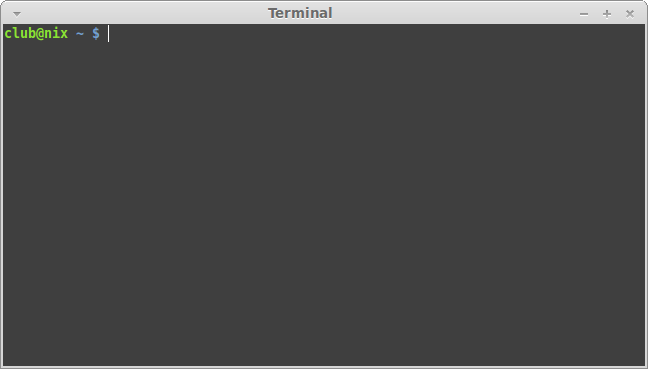
\includegraphics[scale=0.42]{res/Images/terminal}
\end{center}

\newpage
\paragraph{} Le programme qui affiche du texte dans le terminal est ce qu'on
appelle un \emph{Shell}, et il va vous permettre d'entrer des commandes
GNU/Linux. Vous avez aussi l'affichage d'un certain nombre d'informations
utiles:

\begin{enumerate}
	\item[user@pc] correspond à votre login (nom d'utilisateur, ici
		``user'') suivi du nom de la machine (ici ``pc'') sur laquelle
		vous vous trouvez, le tout est séparé par le caractère ``@''.
	\item[$\sim$] est le dossier courant suivit du caractère ``\$''
		(le dossier $\sim$ est un raccourci vers votre dossier personnel
		\emph{/home/user/}).
	\item[\$] Le dollar signifie juste que vous êtes un utilisateur normal (à
		l'opposition du \emph{\#} qui signifie que vous êtes
		super-utilisateur).
\end{enumerate}

\paragraph{} Il existe toutes sortes de Shell (bash, tcsh, sh, ksh, zsh\dots)
qui ont chacun des fonctionnalités différentes, mais tous permettent d'exécuter
des commandes ou des programmes. Dans le monde réel, \emph{bash} est
l'interpréteur le plus courant, cependant pour une raison obscure, vous
commencerez par défaut votre aventure à l'ESIEE avec \emph{tcsh}.

\paragraph{} Comme \emph{tcsh} est très peu convivial, nous supposerons par la
suite que vous utilisez bash (vous pouvez lancer \emph{bash} à l'intérieur du
terminal en tapant la commande \texttt{bash}).

\paragraph{} En résumé, le Shell correspond au programme qui va interpréter et
exécuter les commandes tapées à l'intérieur de votre terminal. Il est composé
de texte, qui affiche des informations utiles, et d'un champ de texte, qui vous
permet d'entrer des commandes en tapant sur le clavier. C'est donc l'interface
minimale entre l'utilisateur et le système d'exploitation.

\paragraph{} Le Shell est exécuté à l'intérieur d'un terminal, qui est une
application graphique qui permet de faire l'intermédiaire entre les programmes
en mode texte et l'utilisateur.

\part{Notation}

\begin{enumerate}
	\item[\^{}] correspond à la touche ``\emph{Ctrl}'', \^{}C, signfie donc
		qu'il faut appuyer en même temps sur la touche ``Ctrl'' et C (deux
		touches sont enfoncées).
	\item [<super>] correspond à la touche ``super'' honteusement surmontée par
		un logo windows sur la plupart des claviers.
	\item [M-] correspond à la touche ``Meta'', le ``alt'' à côté de la touche
		espace.
\end{enumerate}

\newpage
